\chapter{Visión completa de la arquitectura del sistema}

En la figura \ref{fig:arqfinal} se puede ver como se relacionan los subsistemas, los módulos y las herramientas del sistema. Las flechas finas indican el sentido del flujo de datos entre módulos del mismo subsistema, las flechas gruesas indican el flujo de datos entre subsistemas. Las flechas entre Logstash, Kafka Streams y Apache Kafka son bidireccionales ya que tanto Logstash como Kafka Streams pueden utilizar Apache Kafka como buffer para hacer cálculos parciales. 

\begin{figure}[!htb]
	
	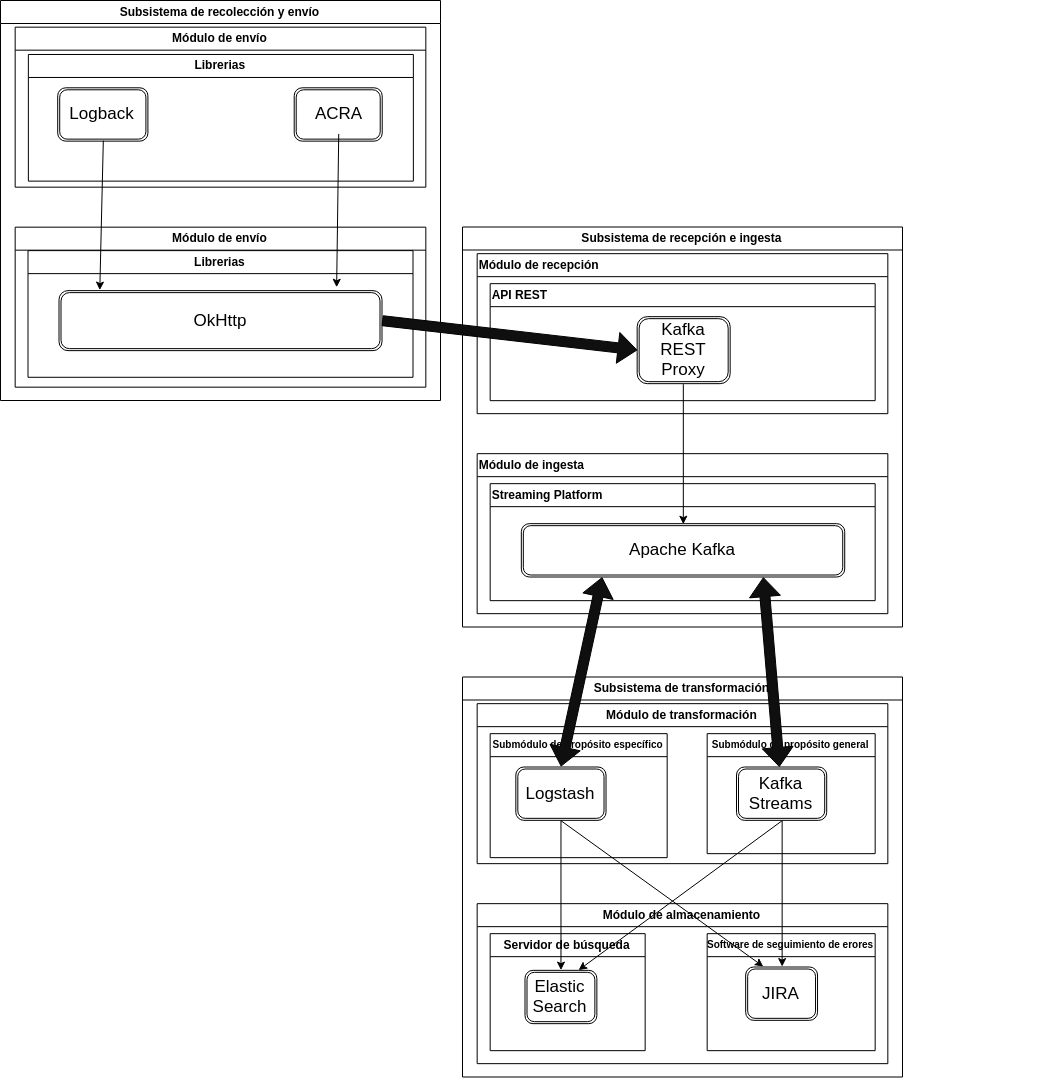
\includegraphics[width=\linewidth] {Moduloss-estructura-todos.png}
	\caption{Visión general de la arquitectura del sistema}
	\label{fig:arqfinal}
\end{figure}